% Tela 1 · Agenda do laboratório (H01 · RF06)
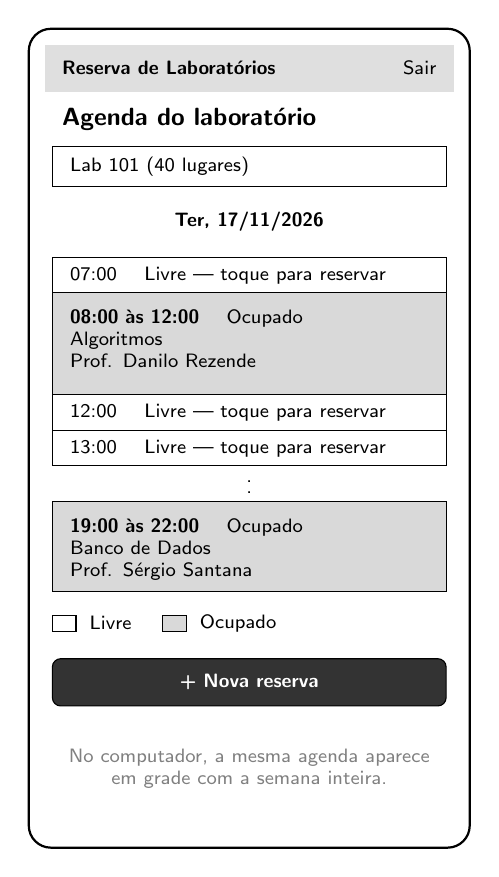
\begin{tikzpicture}[font=\sffamily\scriptsize]
  % aparelho e barra superior
  \draw[thick, rounded corners=8pt] (0,0) rectangle (5.6,10.4);
  \fill[gray!25] (0.2,9.6) rectangle (5.4,10.2);
  \node[anchor=west] at (0.3,9.9) {\textbf{Reserva de Laboratórios}};
  \node[anchor=east] at (5.3,9.9) {Sair};
  \node[anchor=west] at (0.3,9.25) {\small\textbf{Agenda do laboratório}};

  % escolha do laboratório e do dia
  \draw (0.3,8.4) rectangle (5.3,8.9);
  \node[anchor=west] at (0.4,8.65) {Lab 101 (40 lugares)};
  \node[anchor=east] at (5.2,8.65) {$\blacktriangledown$};
  \node at (0.6,7.95) {$\blacktriangleleft$};
  \node at (2.8,7.95) {\textbf{Ter, 17/11/2026}};
  \node at (5.0,7.95) {$\blacktriangleright$};

  % horários do dia
  \draw (0.3,7.05) rectangle (5.3,7.5);
  \node[anchor=west] at (0.4,7.27) {07:00 \quad Livre — toque para reservar};
  \draw[fill=gray!30] (0.3,5.75) rectangle (5.3,7.05);
  \node[anchor=north west, text width=4.8cm] at (0.4,6.95) {\textbf{08:00 às 12:00} \quad Ocupado\\Algoritmos\\Prof. Danilo Rezende};
  \draw (0.3,5.3) rectangle (5.3,5.75);
  \node[anchor=west] at (0.4,5.52) {12:00 \quad Livre — toque para reservar};
  \draw (0.3,4.85) rectangle (5.3,5.3);
  \node[anchor=west] at (0.4,5.07) {13:00 \quad Livre — toque para reservar};
  \node at (2.8,4.62) {$\vdots$};
  \draw[fill=gray!30] (0.3,3.25) rectangle (5.3,4.4);
  \node[anchor=north west, text width=4.8cm] at (0.4,4.3) {\textbf{19:00 às 22:00} \quad Ocupado\\Banco de Dados\\Prof. Sérgio Santana};

  % legenda e botão
  \draw (0.3,2.75) rectangle (0.6,2.95); \node[anchor=west] at (0.65,2.85) {Livre};
  \draw[fill=gray!30] (1.7,2.75) rectangle (2.0,2.95); \node[anchor=west] at (2.05,2.85) {Ocupado};
  \draw[fill=black!80, rounded corners=3pt] (0.3,1.8) rectangle (5.3,2.4);
  \node[white] at (2.8,2.1) {\textbf{+ Nova reserva}};
  \node[text width=5cm, align=center, gray] at (2.8,1.0) {No computador, a mesma agenda aparece\\em grade com a semana inteira.};
\end{tikzpicture}
